\section{An End-to-End Multi-Task and Fusion CNN for Inertial-Based Gait Recognition}

\begin{flushleft}
    \author{
    Rubén Delgrado-Esca$ \tilde{n} $o,
    Francisco M. Castro,
    Julián Ramos Cózar,
    Manuel J. Marín-Jiménez,
    and Nicolás Guil
    }
\end{flushleft}

\begin{center}
    \emph{IEEE DIGITAL OBJECT IDENTIFIER}
\end{center}

\subsection{INTRODUCTION}
An individual's gait appears as their own fingerprint. The study of this 
topic doesn't not only concern the area of medicine, but also that of security 
and identification. The gating study is based on a non-invasive system that 
collects patterns without the direct intervention of the subject. The data, 
which allow the recognition of the gait, are taken by inertial sensors present 
in a multitude of devices such as smartphones or smartwatches. A system 
is presented that uses a convolutional neural network (CNN) that uses the 
data collected by these inertial sensors to be able to predict the subject. The 
approach followed is the one in figure \ref{fig:preview}. Two extensions have been added 
to the network. The first deals with merging sensory data, while the second 
deals with improving the learning process and producing multiple outputs 
from a single input, thanks to a multi-task scheme. The tasks considered 
are: identification, gender recognition and age estimation. The dataset used 
is OU-ISIR gait database \cite{0857651721}.
\begin{figure}[htbp]
    \centering
    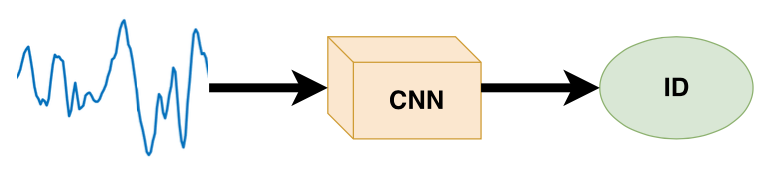
\includegraphics[width = 0.6 \linewidth]{images/paper5/usecase.png}
    \centering
    \caption{A preview of how the model works.}
    \label{fig:preview}
\end{figure}

\subsection{RELATED WORK}
